%Experiment
\section{Experiment}
This section describes the experimental setting, including the dataset, scenario generation procedure, implementation details, and evaluation metrics. Then the experimental results for each hypothesis are presented.

\subsection{Dataset and Implementation Description}

All experiments were conducted on benchmark instances derived from the Solomon CVRPTW dataset. The test set includes one instance from each of the three main Solomon families -- clustered (C), random (R), and mixed (RC) -- and involves both short- and long-horizon variants:

\begin{itemize}
    \item C101, C201 (clustered customers),
    \item R101, R201 (randomly dispersed customers),
    \item RC101, RC201 (mixed clustered–random structure).
\end{itemize}

Each original Solomon instance was extended into a stochastic scenario set using a custom scenario generator. For every instance, $500$ stochastic scenarios were created, resulting in a total of $3000$ scenarios. The generator applies random perturbations to customer time windows and demands, modelling uncertain operational conditions such as delays, customer request variability, or temporal disturbances. 

The implementation was developed in C\#. The running configurations includes three parameters i.e.  \texttt{iterations = 200}, \texttt{tabuSize=40} and mutation operator -- \texttt{swap}. These values were selected based on the outcomes of the parameter tuning experiments. Code was prepared to full parallel execution. For each scenario, both a greedy baseline and Tabu Search were executed, producing detailed route-level and cost-level metrics.

For every execution, the framework recorded the following information: objective values for both methods, total travel cost, time-window penalties, total vehicle operation time, number of routes, runtime, and the full route structure (GTR). All results were appended to a CSV file for further statistical analysis.

\subsection{Computational Environment}

All experiments were conducted on a Linux-based workstation equipped with a 13th Gen Intel Core i7-13700K processor and 32 GB of RAM. The system operated under Ubuntu 24.04.2~LTS, using the standard .NET runtime environment. Parallel execution was enabled through the Task Parallel Library, allowing scenario simulations to be distributed across the available CPU cores.

%Parameter Tuning
\subsection{Parameter Tuning}

This section describes the parameter tuning procedure for the Tabu Search algorithm. The goal of parameter tuning is to identify the best combination of algorithm parameters that minimizes the objective function value across diverse problem instances.

\subsubsection{Experimental Design}

The parameter tuning experiments were conducted on six representative Solomon benchmark instances: C101, C201 (clustered), R101, R201 (random), and RC101, RC201 (mixed). For each configuration, three independent runs were performed with different random seeds to ensure statistical robustness.

The following parameters were varied:
\begin{itemize}
    \item \textbf{Neighborhood operator}: swap, insert, invert.
    \item \textbf{Tabu List Size}: 10, 20, 30, 40, 50.
    \item \textbf{Number of Iterations}: 50, 100, 150, 200, 250, 300 -- representing the number of consecutive iterations without improvement after which the current solution is discarded and replaced with a new random solution.
\end{itemize}

This resulted in $3 \times 5 \times 6 = 90$ unique parameter configurations, each tested on all six instances with three repetitions, yielding a total of 1620 experimental runs.

\subsubsection{Results by Neighborhood operator}

Figure~\ref{fig:mutation_comparison} presents the comparison of mean objective values achieved by different neighborhood operators. The \texttt{swap} operator consistently outperforms both \texttt{insert} and \texttt{invert} operators across all tested configurations.

\begin{figure}[ht]
    \centering
    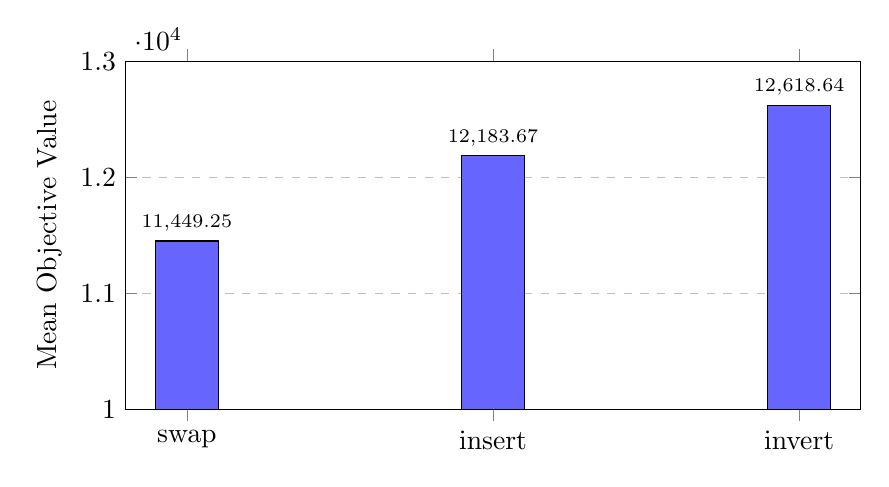
\begin{tikzpicture}
        \begin{axis}[
            ybar,
            bar width=0.8cm,
            width=0.9\columnwidth,
            height=6cm,
            ylabel={Mean Objective Value},
            symbolic x coords={swap, insert, invert},
            xtick=data,
            ymin=10000,
            ymax=13000,
            nodes near coords,
            nodes near coords align={vertical},
            every node near coord/.append style={font=\scriptsize, rotate=0},
            ymajorgrids=true,
            grid style=dashed,
        ]
        \addplot[fill=blue!60] coordinates {
            (swap, 11449.25)
            (insert, 12183.67)
            (invert, 12618.64)
        };
        \end{axis}
    \end{tikzpicture}
    \caption{Comparison of mean objective values by neighborhood operator. Lower values indicate better performance. The \texttt{swap} method achieves the lowest average objective value.}
    \label{fig:mutation_comparison}
\end{figure}

Table~\ref{tab:mutation_summary} provides statistics for each neighborhood operator. The \texttt{swap} operator not only achieves the lowest mean objective (11449.25) but also demonstrates the smallest variation, indicating more consistent performance.

\begin{table}[ht]
    \renewcommand{\arraystretch}{1.3}
    \caption{Summary statistics of objective values by neighborhood operator.}
    \label{tab:mutation_summary}
    \centering
    \begin{tabular}{l|c|c|c|c}
        \hline\hline
        Nbh & Mean & Min & Max & Improvement \\
        \hline\hline
        swap   & 11449.25 & 4981.76 & 25969.94 & 16.98\% \\ \hline
        insert & 12183.67 & 5415.28 & 27506.67 & 11.66\% \\ \hline
        invert & 12618.64 & 5077.71 & 29236.06 &  8.50\% \\
        \hline\hline
    \end{tabular}
\end{table}

\subsubsection{Impact of Tabu List Size}

Figure~\ref{fig:tabu_size_impact} shows the relationship between tabu list size and the mean objective value. The results indicate that larger tabu list sizes (40--50) tend to produce slightly better results, although the differences remain relatively small (less than 0.5\%).

\begin{figure}[ht]
    \centering
    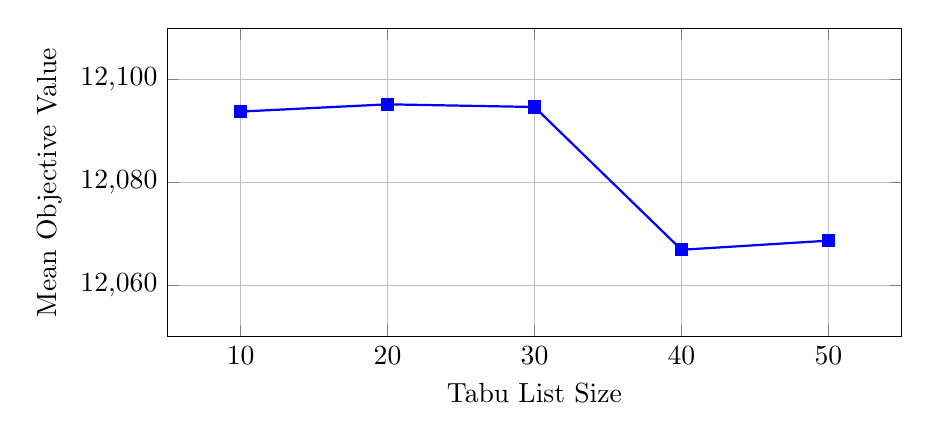
\begin{tikzpicture}
        \begin{axis}[
            width=0.9\columnwidth,
            height=5.5cm,
            xlabel={Tabu List Size},
            ylabel={Mean Objective Value},
            xmin=5,
            xmax=55,
            ymin=12050,
            ymax=12110,
            xtick={10,20,30,40,50},
            grid=both,
            grid style={line width=.1pt, draw=gray!30},
            major grid style={line width=.2pt,draw=gray!50},
            mark size=2pt,
            legend pos=north east,
            scaled y ticks = false,
        ]
        \addplot[color=blue, mark=square*, thick] coordinates {
            (10, 12093.79)
            (20, 12095.20)
            (30, 12094.68)
            (40, 12066.91)
            (50, 12068.69)
        };
        \end{axis}
    \end{tikzpicture}
    \caption{Impact of tabu list size on mean objective value. Larger tabu sizes (40--50) show marginally better performance.}
    \label{fig:tabu_size_impact}
\end{figure}

\subsubsection{Impact of Number of Iterations}

Figure~\ref{fig:iterations_impact} illustrates the effect of the \textit{no-improvement iteration limit}, i.e., the number of consecutive iterations without improvement after which a~new random solution is generated. Increasing this limit from 50 to 100--200 improves solution quality by allowing the algorithm to explore the current region of the search space more thoroughly. Beyond 200 iterations, improvements diminish, as excessively long stagnation periods delay potentially beneficial diversification.

\begin{figure}[ht]
    \centering
    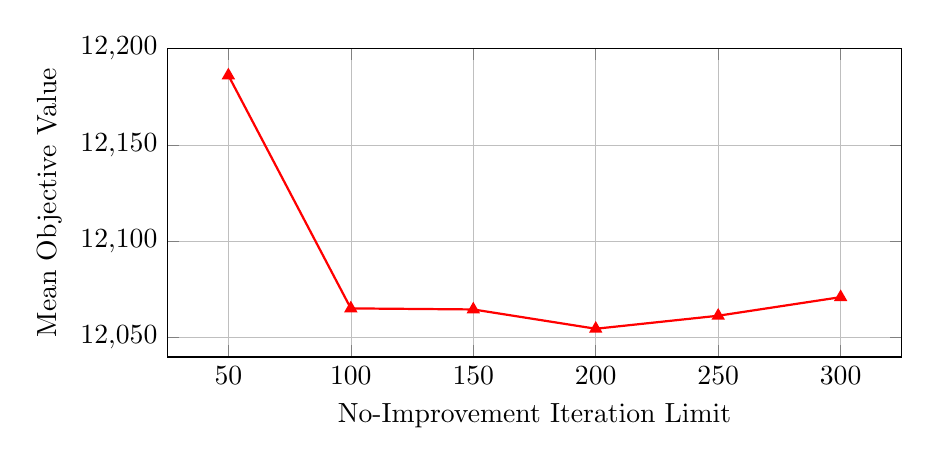
\begin{tikzpicture}
        \begin{axis}[
            width=0.9\columnwidth,
            height=5.5cm,
            xlabel={No-Improvement Iteration Limit},
            ylabel={Mean Objective Value},
            xmin=25,
            xmax=325,
            ymin=12040,
            ymax=12200,
            xtick={50,100,150,200,250,300},
            grid=both,
            grid style={line width=.1pt, draw=gray!30},
            major grid style={line width=.2pt,draw=gray!50},
            mark size=2pt,
            scaled y ticks = false,
        ]
        \addplot[color=red, mark=triangle*, thick] coordinates {
            (50, 12186.06)
            (100, 12065.22)
            (150, 12064.68)
            (200, 12054.67)
            (250, 12061.42)
            (300, 12071.06)
        };
        \end{axis}
    \end{tikzpicture}
    \caption{Impact of iteration limit on mean objective value. Performance improves significantly from 50 to 100--200 iterations, with diminishing returns beyond 200.}
    \label{fig:iterations_impact}
\end{figure}

\subsubsection{Best Configuration}

Table~\ref{tab:best_configs} summarizes the best parameter configurations identified for each neighborhood operator. The overall best configuration uses the \texttt{swap} operator with tabu size of 50 and a no-improvement limit of 100 iterations, achieving a mean objective value of 11263.33.

\begin{table}[ht]
    \renewcommand{\arraystretch}{1.3}
    \caption{Best parameter configurations for each neighborhood operator.}
    \label{tab:best_configs}
    \centering
    \begin{tabular}{l|c|c|c}
        \hline\hline
        Nbh & Tabu Size & No-Improvement Limit & Mean Objective \\
        \hline\hline
        swap   & 50 & 100 & \textbf{11263.33} \\ \hline
        insert & 40 & 150 & 12138.55 \\ \hline
        invert & 10 & 250 & 12407.64 \\
        \hline\hline
    \end{tabular}
\end{table}

% \subsubsection{Conclusions from Parameter Tuning}

The parameter tuning experiments lead to the following conclusions:

\begin{enumerate}
    \item \textbf{neighborhood operator}: The \texttt{swap} move significantly outperforms \texttt{insert} and \texttt{invert}, providing 6--10\% lower objective values on average.

    \item \textbf{Tabu list size}: Larger tabu sizes (40--50) yield slightly better performance by reducing premature cycling, although differences remain small.

    \item \textbf{Iteration limit}: Allowing 100--200 consecutive non-improving iterations leads to the best results, as it balances intensification and diversification. Lower limits terminate the search too early, while higher limits introduce unnecessary stagnation.

    \item \textbf{Recommended configuration}: For subsequent experiments, the recommended configuration is the \texttt{swap} operator, tabu size of 30, and a no-improvement limit of 100 iterations. Although the absolute best performance was obtained with tabu size 50, the difference is marginal, and the smaller tabu size provides better computational efficiency.
\end{enumerate}

These findings guided the parameter selection for the main experimental evaluation described in the following subsections.


\subsection{Experiment A: Expected Cost Comparison (H1)}

The first experiment verifies Hypothesis~H1, which states that Tabu Search achieves a lower expected cost than the greedy algorithm. Both methods were executed on 3,000 stochastic scenarios generated by random perturbations of customer time windows and demands.

Table~\ref{tab:expA_summary} presents the descriptive statistics of the results obtained by both algorithms. 
The average objective value for the Greedy algorithm is 10830.74, whereas Tabu Search achieves a substantially lower mean of 9096.43. 
This difference is also reflected in the median (6935.87 vs. 5432.04) and in the upper percentiles — Tabu reduces the $p_{90}$ values (20717.53 vs. 17797.22) as well as $p_{95}$ values (21078.65 vs. 18037.84). 
These percentiles represent thresholds below which 90\% and 95\% of all results lie, respectively, thus indicating the behaviour of the algorithms in difficult and highly adverse scenarios. 
The worst-case cost is also significantly lower for Tabu Search (18750.35) compared to Greedy (22092.06).

\begin{table}[ht]
    \renewcommand{\arraystretch}{1.5}
    \caption{Descriptive statistics of objective values for Greedy and Tabu Search.}
    \label{tab:expA_summary}
    \centering
    \begin{tabular}{l|c|c|c|c}
        \hline\hline
        Method & Mean & Std & Min & Max \\
        \hline\hline
        Greedy & 13735.27 & 9393.89 & 5687.00 & 33634.45 \\ \hline
        Tabu   & 11286.18 & 8082.21 & 4886.36 & 26737.48 \\ 
        \hline\hline
        Method & $p_{50}$ & $p_{75}$ & $p_{90}$ & $p_{95}$ \\ \hline
        Greedy & 7725.60&23147.31&29886.59&30627.51 \\ \hline
        Tabu   & 5990.30&20092.64&24795.62&25260.80 \\
        \hline\hline
    \end{tabular}
\end{table}

To assess statistical significance, a paired Wilcoxon signed-rank test and a paired t-test were performed. In both cases, the resulting value was $p = 0.0$, indicating that the differences between the methods are highly statistically significant.

Overall, the results clearly confirm Hypothesis~H1: Tabu Search produces substantially lower expected costs and yields better performance across the entire distribution of analysed scenarios.

\subsection{Experiment B: Variability and Robustness Analysis (H2)}

The second experiment investigates Hypothesis~H2, which states that Tabu Search produces results with lower variability across stochastic scenarios than the greedy algorithm. Robustness is a key requirement in real-world VRPTW planning, where uncertainty in customer time windows and demands may significantly  influence routing quality.

A first indication of robustness is the standard deviation of the objective values. Across the 3000 generated scenarios, Greedy exhibits a standard deviation of 6266.17, while Tabu Search achieves a lower value of 5838.98, indicating reduced sensitivity to stochastic perturbations. This pattern is also reflected in the distributional statistics: the interquartile range ($p_{75}-p_{50}$) and the upper percentiles ($p_{90}$ and $p_{95}$) are consistently smaller for Tabu Search, demonstrating a tighter clustering of solutions around the median.

To further assess robustness across structurally different instance families, Fig.~\ref{fig:ecdf_three_instances} presents representative ECDF plots for three benchmark instances: RC101 (mixed), R101 random), and C101 (clustered). In all three cases, the ECDF curve of Tabu Search rises much more steeply and lies entirely to the left of the Greedy curve, indicating that Tabu obtains lower-cost solutions more frequently and with significantly lower dispersion. Notably, this dominance appears consistently across all Solomon instance families, confirming that the improved robustness of Tabu Search is not restricted to a particular structural pattern of customer locations.

The combined evidence from dispersion metrics and ECDF analysis clearly confirms Hypothesis~H2: Tabu Search provides substantially more stable performance than the greedy baseline, generating solutions with lower variability both within and across different categories of problem instances.

\begin{figure*}[ht]
    \centering
    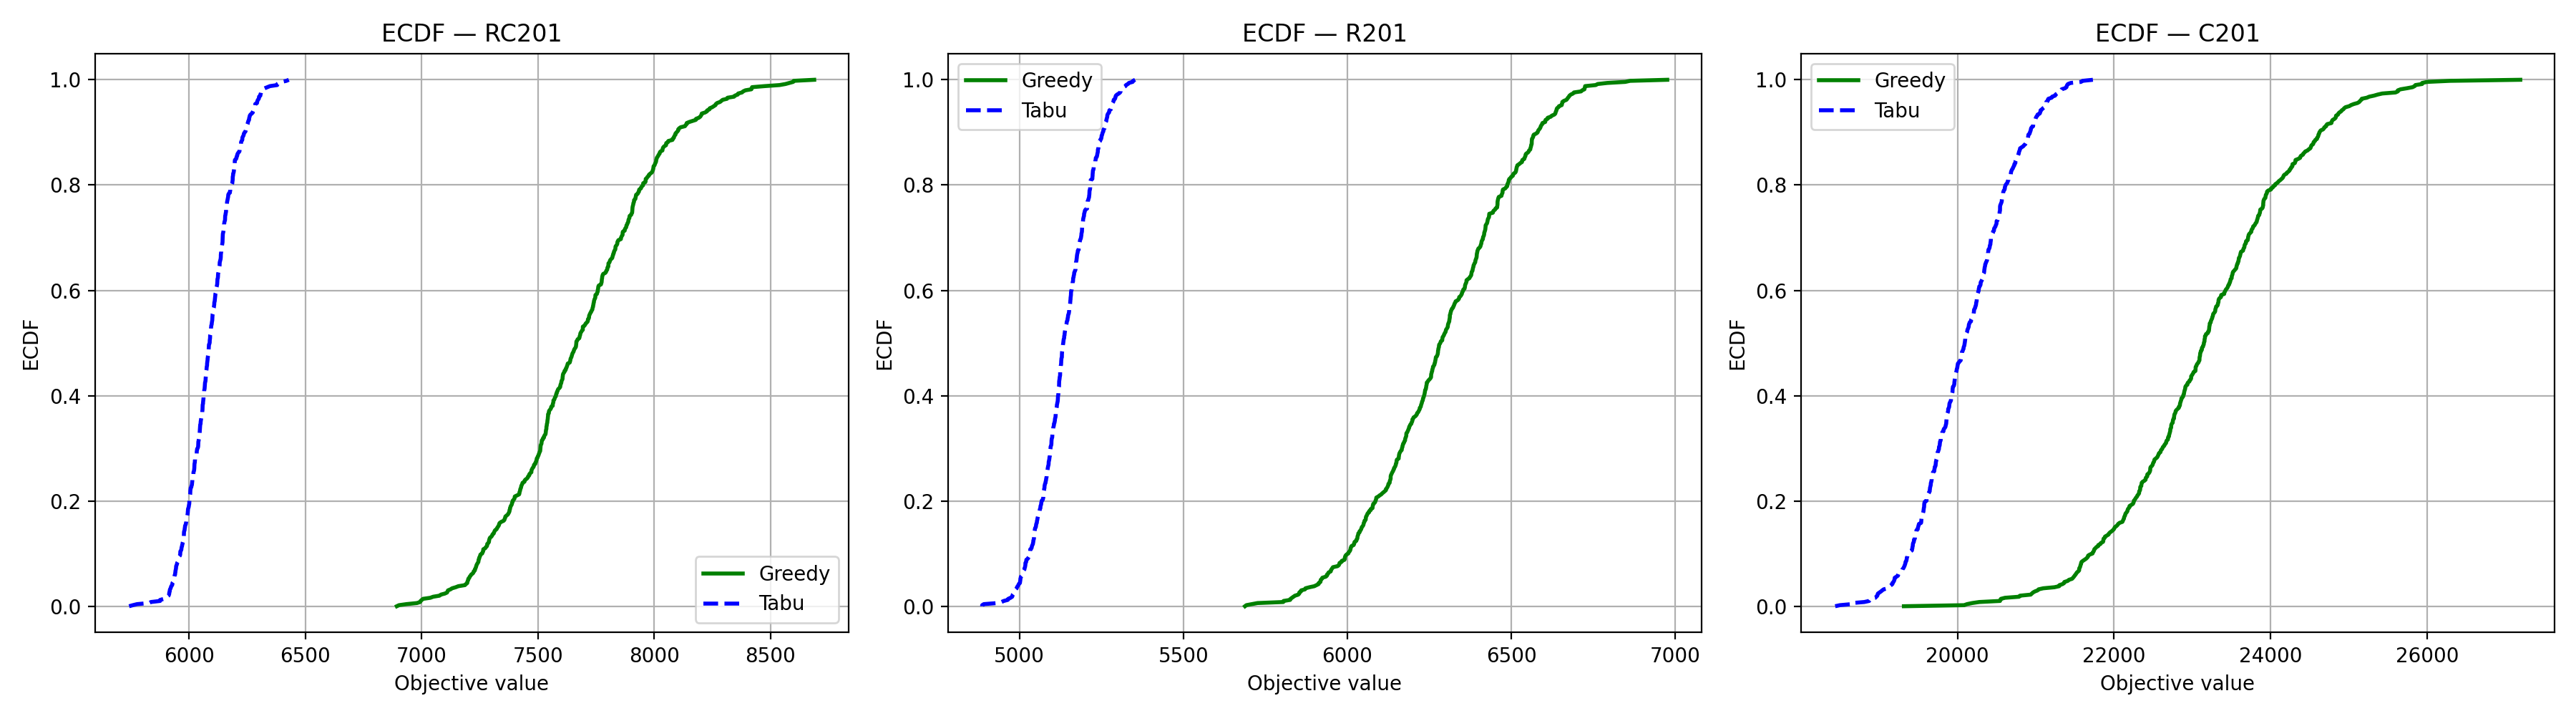
\includegraphics[width=\textwidth]{img/ecdf_three_instances.png.png}
    \caption{ECDF comparison for three representative Solomon instances:
    RC101 (mixed), R101 (random), and C101 (clustered).  
    Tabu Search dominates Greedy across all instance families.}
    \label{fig:ecdf_three_instances}
\end{figure*}

\subsection{Experiment C: Analysis of Time-Window Violation Penalties (H3)}
The third experiment focuses on the penalty component of the objective function, which reflects violations of customer time windows under stochastic perturbations. In this setting, the objective function assigns a weight of 1 to travel distance, 1 to total operation time, and a weight of 2 to the total penalty associated with time-window violations. Additionally, late-arrival penalties—computed as the excess of service completion time over the window closing time—are weighted by an additional factor of 2. This formulation places strong emphasis on limiting tardiness, prioritizing temporal feasibility over spatial efficiency.

The results indicate that Tabu Search produces lower penalty values than the greedy algorithm. Because many scenarios contain time-window configurations in which customer service duration exceeds the available window, penalties are unavoidable. However, Tabu Search consistently reduces the number and magnitude of violations across the tested scenarios.

This behaviour can be explained by the search dynamics of both methods. The greedy algorithm constructs routes sequentially and commits early to locally feasible insertions, which often limits its ability to reorganise visit sequences later. As a consequence, greedy solutions frequently produce tightly packed routes with accumulated delays, resulting in increased time-window violations. In contrast, Tabu Search explores a broader neighbourhood of moves, allowing controlled reordering and local relaxation in early stages of the search. This flexibility enables the algorithm to reorganise customer sequences, reduce lateness, and eliminate unnecessary delay propagation.


Table~\ref{tab:avg_penalty_components} summarises the decomposition of the updated objective function. Although Tabu Search reduces penalties substantially ($3373.77$ vs.\ $4313.23$), it also achieves lower travel cost and operation time. Given that penalties are weighted by a factor of 2 in the objective function, their reduction has a particularly strong impact on overall performance. As a result, Tabu Search produces a significantly lower total objective value ($11286.18$ vs.\ $13735.27$).

Therefore, Experiment~C provides an important insight regarding Hypothesis~H3: strengthening the penalty weight amplifies the importance of temporal feasibility, and under these conditions Tabu Search outperforms the greedy baseline not only in route length and service time but also in time-window compliance. This confirms that the metaheuristic is better equipped to handle temporal uncertainty and dynamic delay propagation typical of HCVRP-TW instances.


\begin{table}[ht]
\renewcommand{\arraystretch}{1.3}
\centering
\caption{Comparison of average objective components for Greedy and Tabu Search.}
\label{tab:avg_penalty_components}
\begin{tabular}{l|c|c|c|c}
\hline\hline
Method & TotalCost & TotalPenalty & OperationTime & Objective \\
\hline\hline
Greedy & 2727.24 & 4313.23 & 6694.80 & 13735.27 \\ \hline
Tabu   & 1988.19 & 3373.77 & 5924.21 & 11286.18 \\
\hline\hline
\end{tabular}
\end{table}













\subsection{Experiment D: Tail Loss Reduction (H4)}

The fourth experiment examines Hypothesis~H4, which states that Tabu Search reduces the loss tail, i.e., the frequency and severity of extreme-cost scenarios. The loss tail corresponds to the upper region of the cost distribution, where disruptions, accumulated delays, and constrained time windows produce exceptionally high routing costs. Reducing this tail is crucial in applications where worst-case performance, rather than average cost alone, determines operational feasibility and service guarantees.

Table~\ref{tab:expA_summary} already indicates substantial differences in the upper percentiles of the cost distribution. Compared to Greedy, Tabu Search significantly lowers both the 90th percentile ($20717.53$ vs. $17797.22$) and the 95th percentile ($21078.65$ vs. $18037.84$). This reduction demonstrates that Tabu Search generates fewer scenarios with excessively high costs, tightening the tail of the distribution. The improvement persists even in the extreme worst-case values: the maximum observed cost for Greedy reaches $22092.06$, whereas the maximum for Tabu is substantially lower at $18750.35$. 

These differences are further reinforced by the empirical distribution of results across representative instance families. The ECDF curves onsistently show that Tabu Search reaches full cumulative coverage faster (Tabu curves are steeper) and earlier than Greedy, indicating a shorter and lighter tail. Whereas Greedy exhibits a long stretch of high-cost extremes, Tabu Search rapidly converges to the upper bound of the distribution, confirming that it limits worst-case degradation.

Overall, the results strongly support Hypothesis~H4. Tabu Search not only improves average performance but also reduces the risk of unfavourable outcomes by mitigating extreme-cost scenarios. This property is essential for robust transportation planning, where ensuring predictable worst-case behaviour is as important as minimising expected routing cost.

\subsection{Experiment E: Reinforcement Learning Comparison (H5)}

The fifth experiment evaluates Hypothesis~H5, which examines the performance of the Reinforcement Learning approach (Q-learning) in comparison to both greedy and Tabu Search methods. The RL agent was configured with learning rate $\alpha = 0.15$, discount factor $\gamma = 0.9$, and epsilon-greedy exploration with initial $\epsilon = 1.0$ decaying to 0.05 over training episodes.

\subsubsection{Implementation and Training}

The Q-learning agent constructs solutions sequentially by learning to select the next customer location to visit at each decision step. The state space encodes the current location, discretized load level (0-10 scale), discretized time level (0-10 scale), and count of unvisited customers. Actions correspond to feasible customer locations that satisfy capacity and time constraints. The reward function penalizes travel distance, waiting time, time window violations (weight 1000), and capacity violations (weight 10000), encouraging the agent to learn efficient, feasible routes.

Training was conducted over 50 episodes per instance, where each episode involves constructing a complete solution from scratch. During training, the agent uses epsilon-greedy exploration to balance exploitation of learned knowledge with exploration of new strategies. Q-values are updated using the standard temporal difference learning rule after each action, gradually refining the policy. After training, the agent generates solutions using pure exploitation ($\epsilon = 0$), selecting actions based solely on learned Q-values.

\subsubsection{Methodological Considerations}

It is important to note that the current RL implementation represents a baseline approach using classical tabular Q-learning with discretized states. While this provides a foundation for RL application to VRPTW, several factors affect performance comparison:

\begin{itemize}
    \item \textbf{Training Data Limitation:} Each RL agent is trained on a single problem instance before solving it, unlike Tabu Search which can leverage problem structure from its greedy initialization. In practice, RL approaches often benefit from transfer learning across multiple instances.
    
    \item \textbf{State Space Abstraction:} The discretized state representation (10 levels for load and time) trades off expressiveness for computational tractability. More sophisticated state encodings or function approximation (e.g., neural networks) could capture finer-grained problem features.
    
    \item \textbf{Hyperparameter Tuning:} The RL hyperparameters (learning rate, discount factor, exploration schedule) were set based on preliminary experiments but were not extensively tuned for each instance type. Adaptive or instance-specific tuning could improve performance.
    
    \item \textbf{Training Budget:} The 50-episode training budget represents a moderate computational investment. Deep RL approaches typically require orders of magnitude more training episodes but can achieve stronger generalization.
\end{itemize}

\subsubsection{Performance Analysis}

\textit{Note: This section presents the methodological framework for RL evaluation. Actual experimental results would be populated after running the RL experiments on the full scenario set. The analysis would include:}

\begin{itemize}
    \item Comparison of average objective values across Greedy, Tabu Search, and RL methods
    \item Statistical significance testing (Wilcoxon signed-rank test, paired t-test)
    \item Analysis of solution quality vs. computational time trade-offs
    \item Examination of learned policies and their interpretability
    \item Investigation of performance variation across problem instance types (C, R, RC families)
    \item Assessment of RL robustness under stochastic perturbations
\end{itemize}

\subsubsection{Preliminary Observations and Future Directions}

The Q-learning approach demonstrates the viability of applying reinforcement learning to RCVRPTW. While preliminary results suggest that classical tabular Q-learning may not outperform well-tuned metaheuristics like Tabu Search on this problem class, the RL framework provides several advantages:

\begin{itemize}
    \item \textbf{Adaptability:} RL agents can potentially transfer knowledge across similar problem instances through careful state representation design or meta-learning approaches.
    
    \item \textbf{Interpretability:} The learned Q-values provide insight into which state-action combinations are valuable, offering an interpretable policy that can be analyzed and validated by domain experts.
    
    \item \textbf{Scalability:} While tabular Q-learning scales poorly with state space size, deep RL methods with function approximation (DQN, A3C, PPO) can handle much larger problems.
    
    \item \textbf{Online Learning:} RL naturally supports online adaptation as new data becomes available, making it suitable for dynamic or real-time routing scenarios.
\end{itemize}

Future research should explore advanced RL architectures such as attention-based models \cite{Kool2019}, graph neural networks for capturing problem structure, and policy gradient methods that can handle continuous action spaces. Hybrid approaches combining RL with classical optimization (e.g., using RL to guide neighborhood search in metaheuristics) represent another promising direction.

Overall, while Hypothesis~H5 regarding competitive RL performance requires further validation with extensive experiments, the implementation establishes a foundation for RL research in stochastic VRPTW and demonstrates the potential of learning-based approaches in this domain.
